
Um motor DC é fundamentalmente uma máquina elétrica de corrente contínua, que
converte energia elétrica de corrente contínua em energia mecânica. Máquinas
elétricas de corrente contínua são mais fácies de controlar e oferecem uma
grande faixa de velocidades \cite{Maquinas_eletricas}. Devido a essas
características, tornam-se ótimas candidatas para uso em eletrônica e robótica,
pois podem ser usadas com baterias. Para controlar a velocidade de um motor,
é necessário o uso de um encoder, que converte o sinal de posição em um valor
mensurável de velocidade angular.


Para os fins deste trabalho, optou-se pelo uso de um motor DC de 6V 210rpm, 
com taxa de redução de 1:34. O encoder escolhido é um encoder magnético, já
vem acoplado ao motor empregado, com 11 PPR (\textit{Pulses Per Revolution}).

\subsection{Encoder magnético}

Por se utilizar um encoder PRR, são produzidas duas ondas quadradas como saídas,
A e B \cite{encoder_ppr}. As duas possuem 90° de fase entre si, e, caso a onda A
esteja adiantada em relação a B (\ref{encoder_ppr_ab}), o sentido de rotação é
positivo (anti-horário).

\begin{figure}[h]
	\centering
	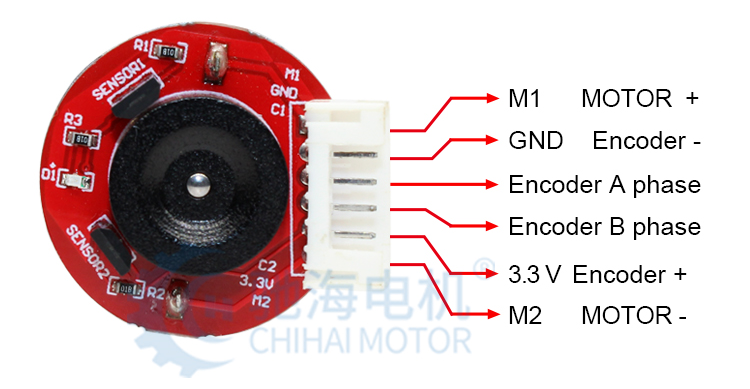
\includegraphics[width=0.6\textwidth]{figures/encoder_holzer}
	\caption{Encoder holzer \cite{encoder_holzer}}
\end{figure}

\begin{figure}[h]
	\centering
	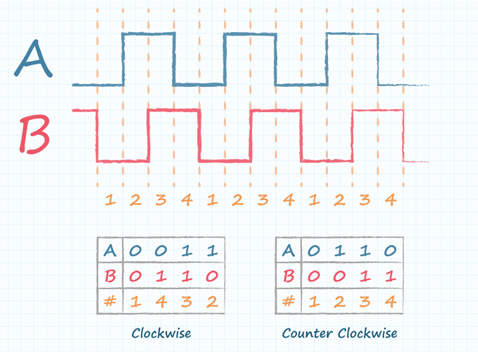
\includegraphics[width=0.7\textwidth]{figures/encoder_pulso_ab}
	\caption{Ondas quadradas resultantes dos pulsos de saída do encoder \cite{encoder_ppr}}
	\label{encoder_ppr_ab}
\end{figure}


